\documentclass[a4paper,11pt]{article}
\usepackage{amsmath,amssymb}
\usepackage[a4paper,left=19mm,right=19mm,top=40mm,bottom=40mm]{geometry}
\usepackage{txfonts}
\usepackage{kotex}
\usepackage{graphicx}
\usepackage{algorithm}
\usepackage{algpseudocode}
\usepackage{fancyvrb}

\begin{document}
\title{자료구조 HW5}
\author{B935394 컴퓨터공학과 장준희}
\maketitle
\newpage
\section{코드 설명}
우선 리스트(generalized list,GenList) 의 구조는 다음 그림과 같다.\\
\begin{figure}[h]
\begin{center}
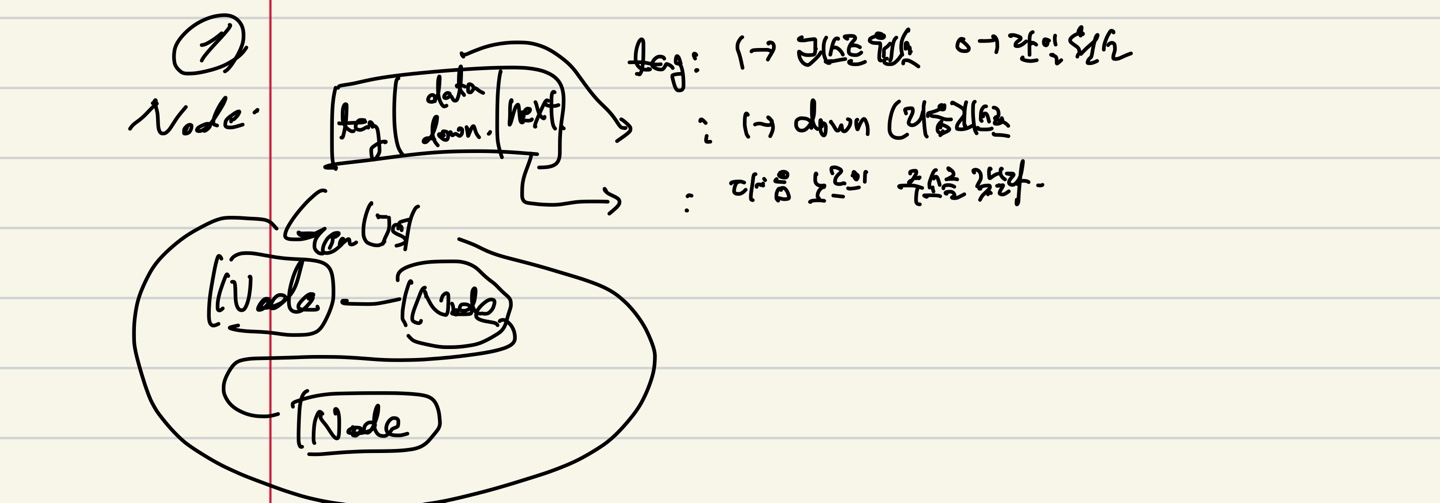
\includegraphics[width=0.7\textwidth]{struct}
\caption{구조}
\label{fig:fig1}
\end{center}
\end{figure}
\newline
GenList를 만드는 Make함수부터 살펴보면, 다음 그림과 같다.
\begin{figure}[h]
\begin{center}
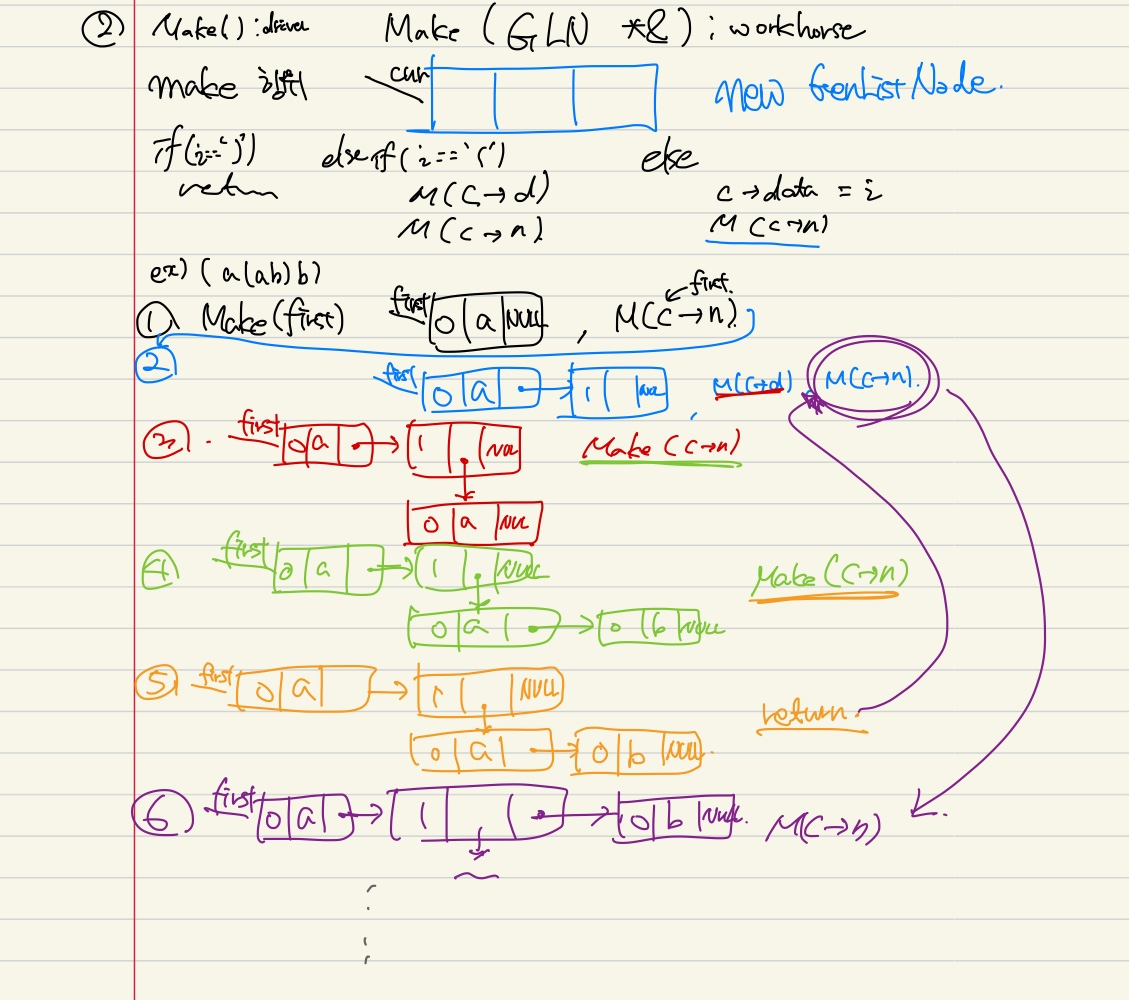
\includegraphics[width=0.6\textwidth]{make}
\caption{Make}
\label{fig:fig2}
\end{center}
\end{figure}
\\우선 Make라는 행위는 현재의 cur이라는 포인터에게 새로운 객체를 가리키게끔 해주는 것이다.(cur = new ~~)
Make함수에서 처리해야할 경우는 3가지가 있는데 입력이 각각 ')', '(', 어떤 문자인 경우이다. 각각을 살펴보면,
\begin{itemize}
\item ')' : 단순히 return만 해주면 된다.
\item '(' : cur이 가리키는 노드의 tag에 1을 대입한 후 Make(cur$->$down),Make(cur$->$next)를 해주면 된다. (Fig\ref{fig:fig2}에서 tag=1의 과정을 실수로 빼먹었다.)
\item 어떤 문자 : cur이 가리키는 node의 data에 문자를 대입한 후 Make(cur$->$next)를 해주면 된다.
\end{itemize}
각각의 경우를 살펴보면서 Make함수가 자신의 실행 중에 Make함수를 다시 불러내는 경우가 있음을 볼 수 있다. 이런 경우를 재귀함수라고 한다.  재귀함수의 흐름을 보기 위해서 Fig\ref{fig:fig2}에 간단히 예시를 들고 그 흐름을 그림과 함께 표현하였다. 그 안에서 계속 꼬리를 물어가며, node가 생성되는 것을 알 수 있고, 살펴본 경우 중 '('의 경우에서 Make(cur$->$down),Make(cur$->$next)이라고 해준 덕분에  Make(cur$->$down)에서 내려가서 계속 Make를 해나가다가 return을 하더라도 원래의 노드(tag=1)로 돌아와서 다음 노드를 연결시킬 수 있음을 볼 수 있다. 나머지 Insert, Print, Insert함수도 이러한 재귀 아이디어를 쓰고 있다. Insert나 Print 함수는 cur가 가리키는 노드의 데이터를 본 후 그에 맞춰서 삽입(cur이 가리키는 노드의 next가 가리키는 새로운 노드를 만들어 주고 원래의 next가 가리키던 노드는 새로운 노드의 next가 가리키게 된다.)하거나 출력하면 된다. 실제 코드는 다음과 같다.
\begin{Verbatim}
--------------------------------------------------------------------
void GenList::Print(GenListNode *&cur)
{
    if(cur->tag==false){
        cout<<cur->data;
        if(cur->next!=NULL)
            Print(cur->next);
        else{
            cout<<')';
            return;
        }
    } 
    else if(cur->tag == true){
        cout<<'(';
        if(cur->down!=NULL)
            Print(cur->down);
        else
            cout<<')';        
        if(cur->next!=NULL)        
            Print(cur->next);
        else{
            cout<<')';
            return;
        }
    }
}
--------------------------------------------------------------------
void GenList::Insert(GenListNode *&cur, char i, char j)
{
    if((cur->tag==0)){
        if(cur->data==i){
            GenListNode * newNode;
            newNode=new GenListNode();
            newNode->next=cur->next;
            cur->next=newNode;
            newNode->data=j;
            newNode->tag=0;
        }
        if(cur->next!=NULL)
            Insert(cur->next,i,j);
    }
    else if((cur->tag==1)){
        if(cur->down!=NULL)
            Insert(cur->down,i,j);
        if(cur->next!=NULL)
            Insert(cur->next,i,j);
    }
    if(cur->next==NULL){
        return;
    }
}
--------------------------------------------------------------------
\end{Verbatim}
\newpage
Delete함수는 조금 복잡했는데 설계과정에서는 4가지 정도의 경우면 충분하지 않을까 했으나, 실제로는 더 많은 경우가 필요했다. Fig\ref{fig:fig3}에 Delete가 무엇인지, 각각의 경우에 무엇을 해야하는지를 파란색으로 표현하였다.
 \begin{figure}[h]
\begin{center}
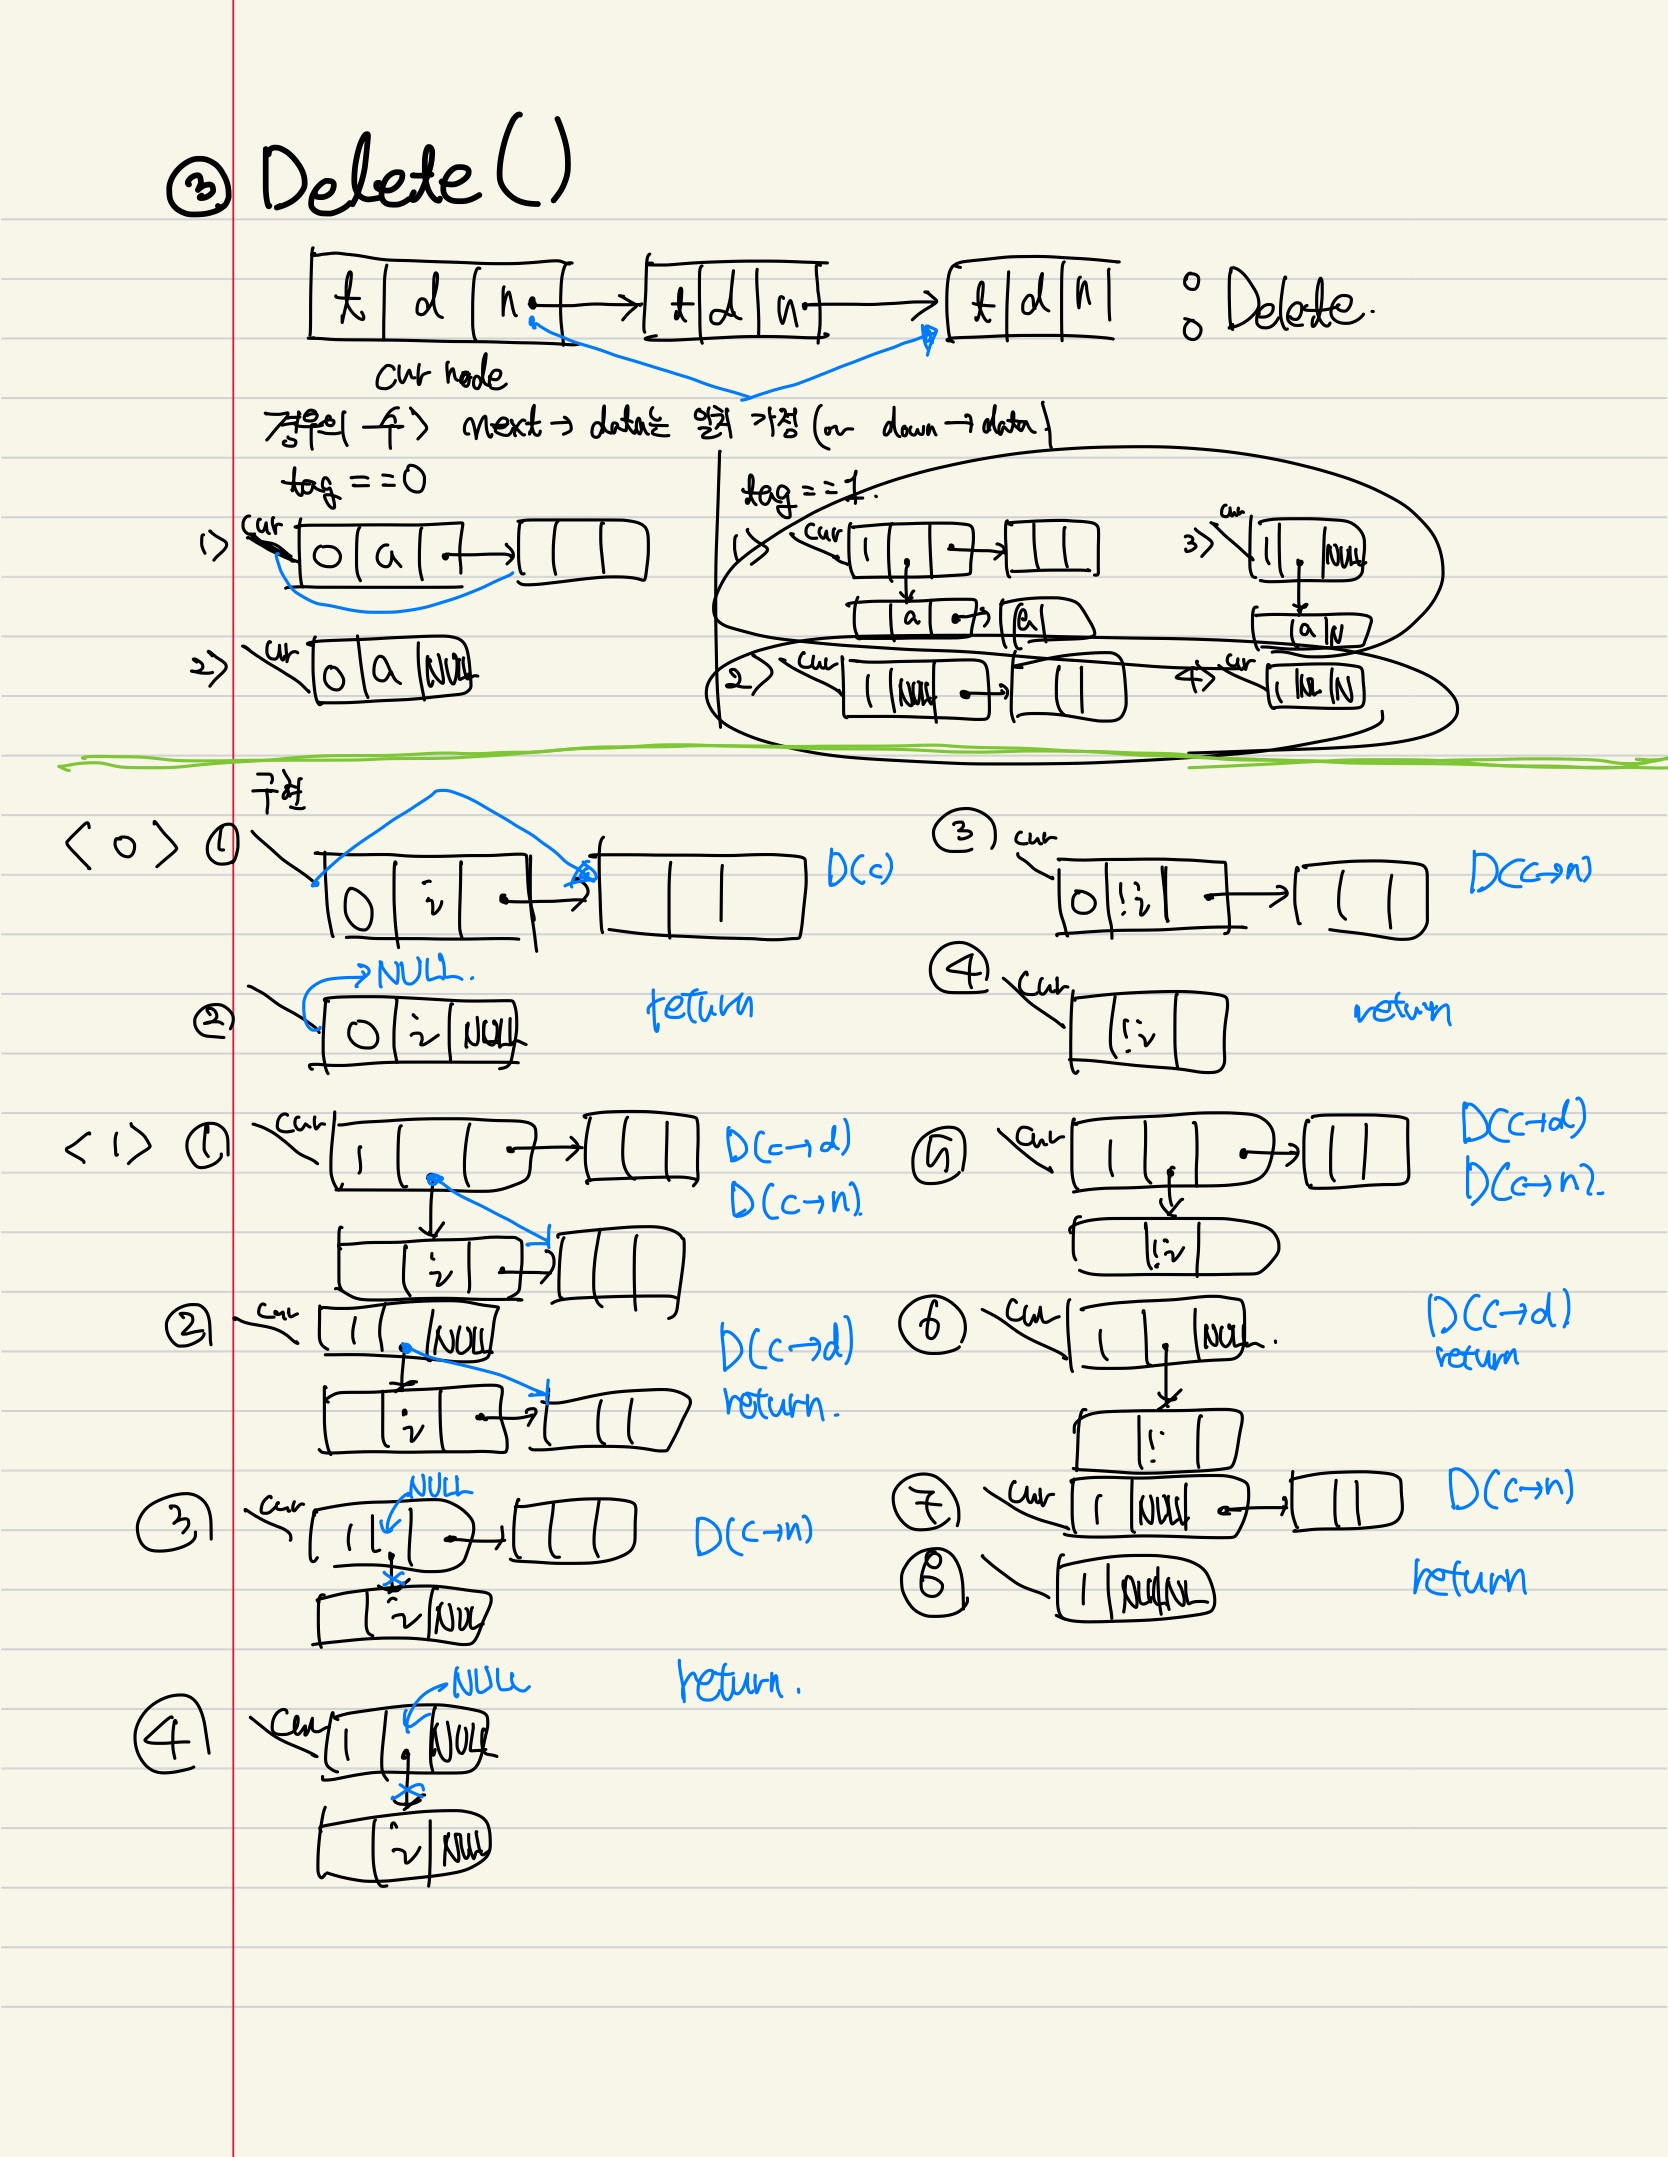
\includegraphics[width=0.7\textwidth]{delete}
\caption{Delete}
\label{fig:fig3}
\end{center}
\end{figure}
\\  $<0>$은 tag==0인 경우 $<1>$은 tag==1인 경우이다.실제 코드는 다음과 같다.\newpage
\begin{Verbatim}
--------------------------------------------------------------------
void GenList ::Delete(GenListNode *&cur, char i)
{    
    if(cur->tag==0){    
        if(cur->data==i){
            if(cur->next!=NULL){
                cur=cur->next;
                Delete(cur,i);
            }
            else{       
                cur=NULL;
                return;
            }
        }
        else{
            if(cur->next!=NULL){
                Delete(cur->next,i);
            }
            else{       
                return;
            }
        }
    }
    else{   //tag=1
        if(cur->down!=NULL){
            if(cur->down->data==i){
                if(cur->down->next!=NULL){
                    cur->down=cur->down->next;
                    Delete(cur->down,i);
                    if(cur->next!=NULL){
                        Delete(cur->next,i);
                    }
                    else
                        return; 
                }
                else{
                    cur->down=NULL;
                    if(cur->next!=NULL){
                        Delete(cur->next,i);
                    }
                    else
                        return;
                }   
            }
            else{
                Delete(cur->down,i);
                if(cur->next!=NULL){
                    Delete(cur->next,i);
                }
                else
                    return; 
            }         
        }
        else{
            if(cur->next!=NULL){
                Delete(cur->next,i);
            }
            else
                return;     
        }
    }
}
--------------------------------------------------------------------
\end{Verbatim}
\section{과제 구현 시 어려웠던 점}
\begin{itemize}
\item cur이 포인터라는 것을 자꾸 망각해서, Delete함수처럼 경우가 많아지고, 복잡해지면 계속 설계하는데 오해를 했다. ($cur->next->data$를 i와 비교하는 등...) 이번 과제를 통해 포인터의 개념을 다시 한 번 상기할 수 잇었고, 과제 pdf를 통해 표현을 어떻게하면 안 헷갈릴 수 있는지 깨닫게 되었다.
\item Print와 Insert구현이 어렵지 않았는데 계속하여 Segmantation Fault가 떠서 열받았던 적이 있다. 디버깅을 한줄한줄 돌리면서 값들을 비교하다보니 Delete를 하는 과정에서 tag가 1이더라도 down이 NULL을 가리킬 수도 있던 것이였다. 조금 더 조심할 필요를 느꼈다.
\item Delete의 경우 원래 설계를 안하고 무작정 만들었었는데, 도무지 답이 안나왔었다. 설계의 중요성을 깨달았다.
\item 과제랑 직접적으로 관련이 있는 것은 아니였지만, 남들도 다 쓴다해서 VScode를 처음 써보기 시작했는데 세팅이 어려웠었다. 구글링을 통해서 세팅을 다 끝마치고 나니, 마음에 들고 뿌듯했다.
\end{itemize}



\end{document}